\documentclass[11pt]{article}
\usepackage{authblk}
\usepackage{eacl2014}
\usepackage{url}
\usepackage{latexsym}

\usepackage{fontspec}
\usepackage{xunicode}
\usepackage{xltxtra}



\setmainfont[Mapping=tex-text]{Times New Roman}

%\setlength\titlebox{6.5cm}    % You can expand the title box if you
% really have to

\title{Optimising Morphological Analyser Transducers Using Morphological Structure
and Automatically Induced Flag Diacritics - Abstract}


\iffalse
\author{Senka Drobac//affff \and Krister Lind\'{e}n/affff \and Tommi A Pirinen//bbbb \and Miikka Silfverberg/affff  \\
Department of Modern Languages \\
PO Box 24 \\
00014 University of Helsinki \\
{\tt \{senka.drobac, krister.linden, tommi.pirinen, miikka.silfverberg\}@helsinki.fi}}
\institute{bla}
\fi


\author[1]{Senka Drobac}
\author[1]{Krister Lind\'{e}n}
\author[2]{Tommi A Pirinen}
\author[1]{Miikka Silfverberg}
\affil[1]{Department of Modern Languages, PO Box 24, 00014 University of Helsinki}
\affil[2]{Department of Speech Sciences, PO Box 9, 00014 University of Helsinki}



\renewcommand\Authands{ and }




\date{\today}

\begin{document}
\maketitle

\section{Rationale}

    Flag diacritics enable optimising finite-state networks by
    combining identical sub-graphs of its transition
    graph. Traditionally, the feature has required linguists to devise
    the optimisations to the graph by hand alongside the morphological
    description. In this paper, we present a novel method of
    discovering flag positions in morphological lexicons automatically
    based on the morpheme structure implicit in the language
    description. With this approach, we have gained significant
    decrease in the size of finite-state networks while maintaining reasonable application speed.

\section{Introduction}

Finite-state transducers are an established way of encoding
morphological analysers for natural languages. Nevertheless,
full-scale morphological analysers can often grow to be too large for
use cases like spell checkers, speech processing and shallow parsing, which 
should have moderate memory footprint. Large transducers can be optimised by recognising
equivalent sub-graphs and combining them by using special symbols called
flag diacritics, to couple entrance points of the sub-graphs with the
correct exit points.

Up to date, applying flag diacritics has required a linguist to provide
the lexicon compiler with their positions. However, there are two
major problems with this kind of approach: Firstly, linguists often do
not have a very good understanding of the structure of the
finite-state networks built from lexicographical-morphological
descriptions; Secondly, the addition of flag diacritics to these
descriptions makes them unreadable and unmanageable since the amount
of non-linguistic data in the linguistic description increases. 

One of the reasons why flag diacritics have been so cumbersome from
the linguists point of view, is their two-fold nature. On one hand,
they are there to optimise the finite-state automaton structure,
e.g. in~\cite{karttunen2006numbers}. On the other hand, they are the
primary method of describing non-contiguous morphological
constraints~\cite{beesley1998constraining}. If they are applied on the
constriction of separated morphotactic dependencies, the effect on
optimisation is at best haphazard, and the resulting description is
neither linguistically motivated nor maintainable from a computational
view-point.

This article seeks to address problems associated with flag diacritics
by using an algorithm for inducing flag positions from the linguistic
morpheme structure, implicitly present in lexical
descriptions.

\begin{figure*}
    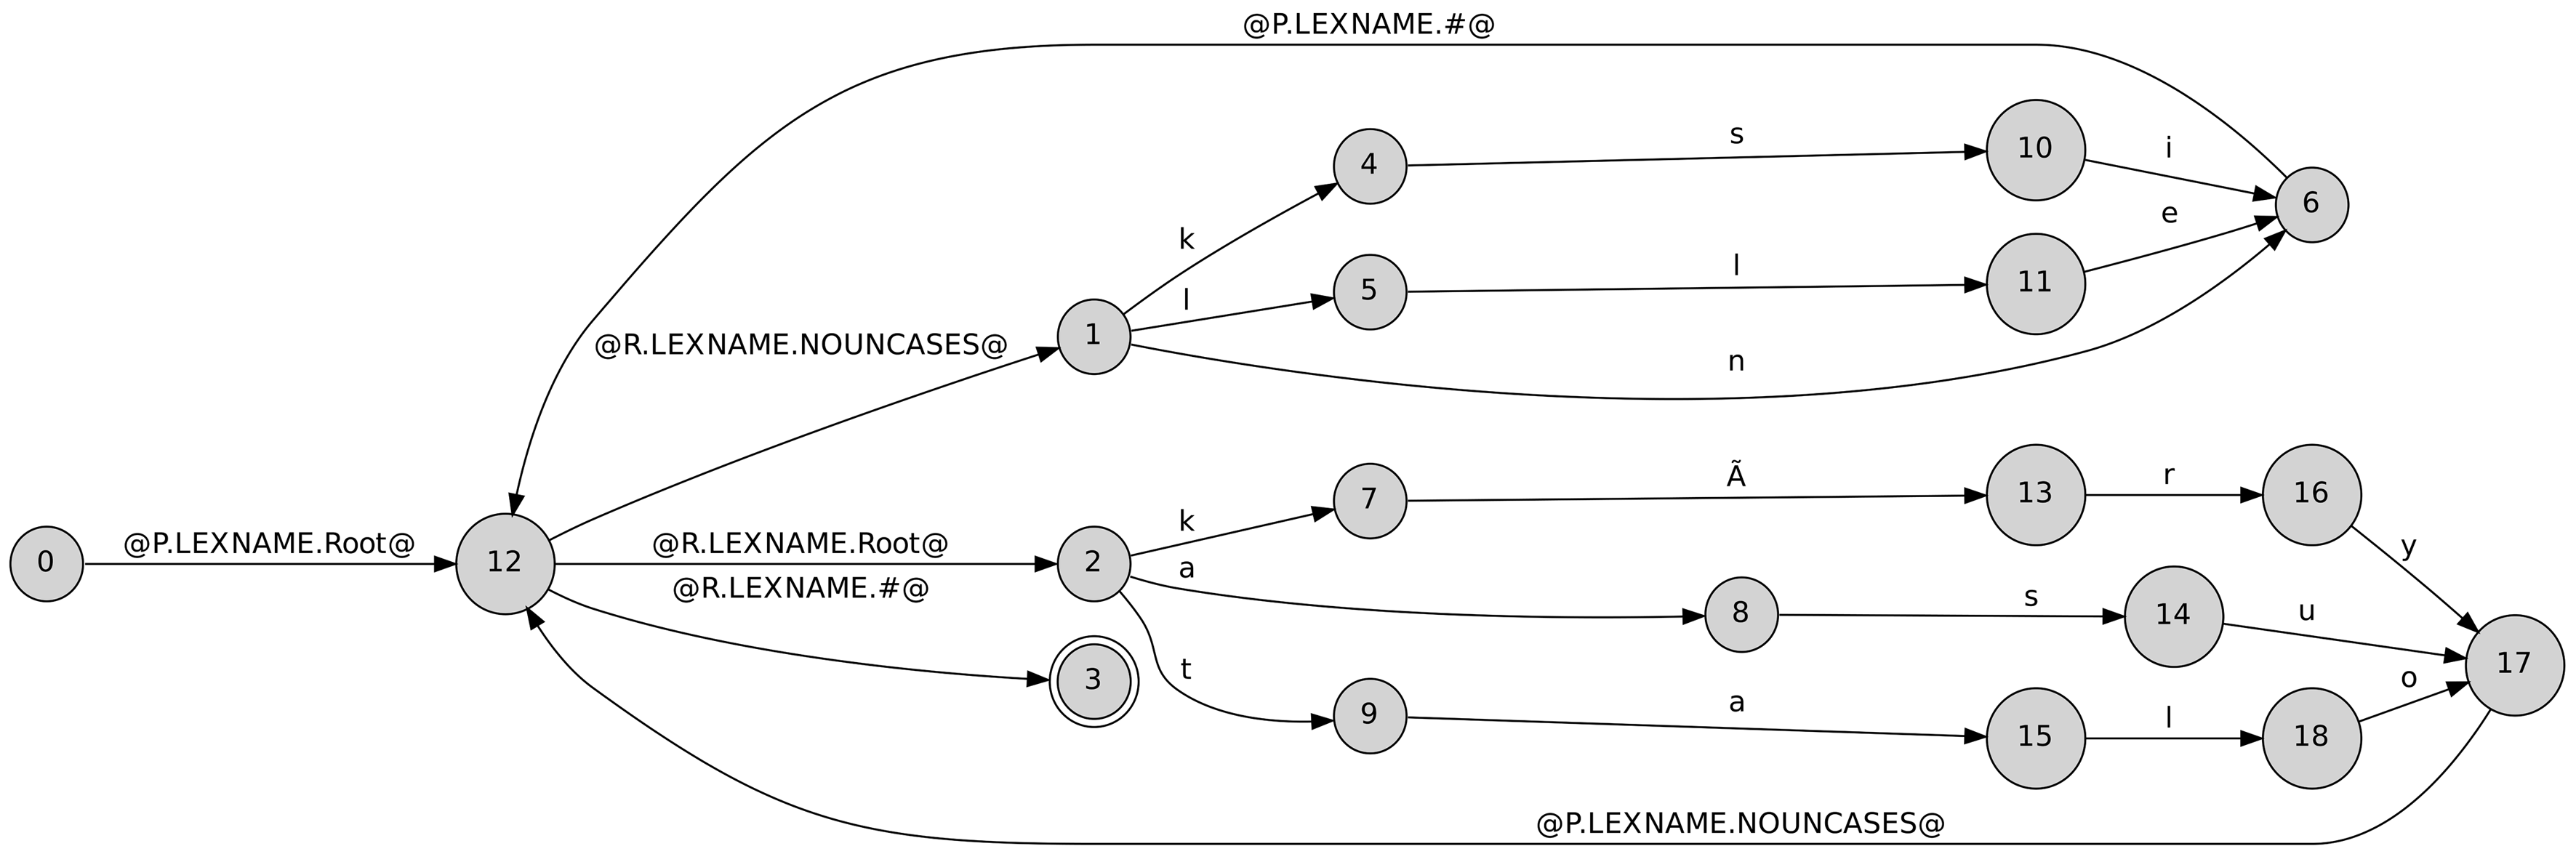
\includegraphics[width=\textwidth]{transducer.png}
     \caption{Simplified part of Finnish lexc grammar description with automatic flags
     \label{fig:lexc-fin-flag}}
\end{figure*}

\begin{figure*}
    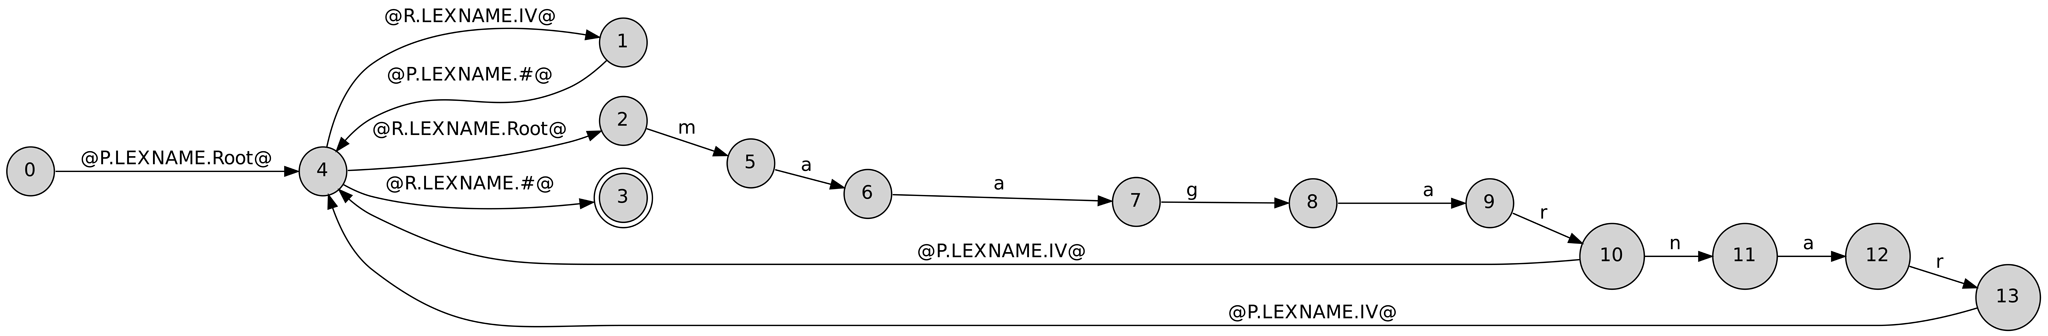
\includegraphics[width=\textwidth]{gr.png}
     \caption{Simplified part of Greenlandic lexc grammar description with automatic flags
     \label{fig:lexc-gr-flag}}
\end{figure*}

\section{Background}

\label{sec:background}

Finite state morphology~\cite{beesley2003finite} is the
state-of-the-art in writing morphological analysers for natural
languages of the whole range of typologically varying morphological
features. The finite-state approach is built around two practical
concepts: constructing lexicographical descriptions of the language
using a syntax called lexc and expressing morphophonological
variations as regular expression rules. In this paper we study the use
of lexicographical structure as framed by lexc. 

Lexc is a simple right-linear phrase structure grammar formalism. In
linguistic terms this means approximately the following: we have
collections of lexicons, which are lists of morphemes. Each morpheme
in a lexicon defines a continuation lexicon, which in turn determines
the set of morphemes that can succeed the original morpheme and their
possible continuations.

Consider for example Finnish morphology. Nominal inflection can be
constructed neatly from left to right. In figure~\ref{fig:lexc-fin},
there is a lexc representation of the Finnish words \emph{talo} `house',
\emph{asu} `clothing' and \emph{kärry} `cart', and nominal suffixes
\emph{n} (singular genitive), \emph{lle} (singular allative) and
\emph{ksi} (singular translative). Derivation of word-forms starts
from the \texttt{Root} lexicon. Each of the nouns in root set of morphemes
continues rightwards to \texttt{NOUNCASES} set of morphemes, and each
case morpheme continues towards the special \texttt{\#} lexicon
signifying the end of a word-form.




\begin{figure}
    \centering
    \begin{verbatim}
    LEXICON Root
    talo NOUNCASES ;
    asu NOUNCASES ;
    kärry NOUNCASES ;

    LEXICON NOUNCASES
    n # ;
    lle # ;
    ksi # ;
    \end{verbatim}
    \caption{Simplified part of Finnish lexc grammar description
    \label{fig:lexc-fin}}
\end{figure}

Finnish was used as an example in Karttunen's paper on flag diacritics
in optimisation~\shortcite{karttunen2006numbers}. In that paper, he
showed that the optimisation quality of wisely selected flag
diacritics can be substantial; from a 20,498 state automaton to an
1,946 state one. The article describes Finnish numerals, which have
the feature of requiring agreeing inflection in free compounding. This
can be achieved by allowing all compounds and restricting the
combinations by flags, instead by lexicon structure. Unfortunately,
the article does not show examples or re-producible description of the
lexicographical data, but to our experience there are no available
morphologies that show similar compression quality, so it can be
considered towards the upper bounds of what such compression can
achieve.
 

\section{Methods}
\label{sec:methods}

Flag diacritics are special multi-character symbols which are interpreted during runtime. They have special syntax: \verb+@operator.feature.value@+, where
\texttt{operator} is one of the available operators (P, U, R, D, N, C), \texttt{feature} is name of a feature provisionally set by user and \texttt{value} can be any value held in feature, also provisionally defined ~\cite{beesley2003finite}.

In this paper, we will use only two types of flag diacritics: positive
setting (\verb+@P.feature value@+) and require test
(\verb+@R.feature value@+). While positive setting flag only sets the
feature to its value, require test flag invokes testing whether the
feature is set to the designated value.  For example,
\verb+@P.LEXNAME.Root@+ will set feature \texttt{LEXNAME} to value
\texttt{Root}. If later in the path there is an R flag that requires test
\verb+@R.LEXNAME.Root@+, the invoked test will succeed and that path
will be considered valid.

Our algorithm is based on the finding that adjacent morph combinatorics can be expressed with finite-state flags like this:

Every rightward continuation is replaced with a positive setting flag
with feature called \texttt{LEXNAME} and value corresponding to the
continuation lexicon. For example, the lexicon in
figure~\ref{fig:lexc-fin} has two rightward continuations:
\texttt{NOUNCASES} and \texttt{\#}, which are represented using flags
\verb+@P.LEXNAME.NOUNCASES@+ and \verb+@P.LEXNAME.#@+.  Similarly,
every leftward continuation is replaced with request test flag which
also has feature \texttt{LEXNAME} and the corresponding
value. Therefore, the lexicon shown in figure~\ref{fig:lexc-fin} will
also have two leftward continuations: \texttt{NOUNCASES} and
\texttt{\#}, which are represented using flags
\verb+@R.LEXNAME.NOUNCASES@+ and \verb+@R.LEXNAME.#@+. Additionally,
every morphological description starts with \texttt{Root}, which is
represented using the pair of flags
\verb+@P.LEXNAME.Root@@R.LEXNAME.Root@+.

The transducer built from the morphological description in
figure~\ref{fig:lexc-fin} is shown in figure~\ref{fig:lexc-fin-flag}.

Since real-world morphological descriptions often contain empty, or nearly
empty, continuation lexicons, inserting flags in those cases only
increase size of the transducer, without gaining any
benefits. Therefore, those continuation lexicons are recognized
during compilation time and skipped when inserting corresponding flag
diacritics.


% Here should come part with automatically finding which flags not to insert (P1, P2, P3?)

Lexicons that contain flag diacritics can be composed with other
transducers which also contain flag diacritics without worrying about
flag collisions. This is achieved by renaming flag diacritics in both
argument transducers in such a way that collisions become impossible
and then inserting flag diacritics freely from each argument to the
other.

Consider for example composition of a lexicon $L$ with a rule $R$. If
both transducers contain flag diacritics for feature {\tt FEATURE},
then $all features F$ are renamed {\tt F1} in $L$ and {\tt F2} in
$R$.~\footnote{It is not sufficient to rename only flag diacritics
  with common features, because that might clash with existing feature
  names.} All flag diacritics (like {\tt @P.F.True@}) are renamed
correspondingly (to {\tt @P.F1.True@} in $L$ and {\tt @P.F2.True@} in
$R$) and a new lexicon $L'$ and rule $R'$ are created by inserting
freely all flag diacritics from $R$ to $L$ and from $L$ to $R$.

The transducers $L'$ and $R'$ can be composed and it is easy to
see that the result satisfies the property that, if flag diacritics
are compiled out, then the resulting transducer without flag
diacritics will accept exactly the same strings as the composition of
the transducers that are obtained by compiling out flag diacritics
from the original lexicon $L$ and the original rule $R$.

In table~\ref{table:sizes} there are shown sizes of the original
transducers compiled with regular lexc compiler composed with grammar rules, transducers compiled
with new method that inserts flag diacritics composed with grammar rules and finally their ratio.

\begin{table}
    \centering
    \begin{tabular}{|l|r|r|r|}
        \hline
        \bf Language & \bf Original & \bf With flags & \bf \% \\
        \hline
        \bf Greenlandic &   168   & 17 & 10,1\%  \\
        \bf North Saami &   12     & 5,7 & 47,5\%  \\
        \bf Lule Saami  &   5     & 3 & 60,0\%  \\
        \bf Erzya       &   3,7     & 5,3 & 143,2\%  \\
        \hline
    \end{tabular}
    \caption{Sizes of transducers without and with automatic flags (in megabytes); Percentage shows size of the flagged transducer in comparison to the original
    \label{table:sizes}}
\end{table}

% Add pruning flags!!!


% Find out and discuss why tr with lots of flags get big after applying rules

\section{Data}
\label{sec:data}

We measure the success of our algorithm using real-world, large scale
language descriptions. For this purpose we have acquired freely
available, open source language descriptions from University of
Tromsa's language repository~\cite{moshagen2013building}.\footnote{https://victorio.uit.no/langtech, revision 73836} The
languages selected are Greenlandic (kal), North Saami (sme), Erzya
(myv), and Lule Sami (smj).

All operations with transducers were performed using Helsinki Finite
State Technology tools~\cite{linden2011}.



\section{Discussion}
\label{sec:discussion}

The results of this study show that large scale language descriptions
can be compiled into smaller transducers using automatically inserted
flags. The effect is especially pronounced for language descriptions
which repeat morphemes in many different places, like the
morphological analyzer for Greenlandic. Since flag diacritics
themselves take space in the transducer graph, this method did not
offer improvements for descriptions where the original
transducer was small.

While requiring {\tt R} flag diacritics will always occur only once
for every left continuation lexicon, the results have shown that, for
certain right continuations, P flag diacritics occur hundreds of
times. This will happen every time when in the same set of morphemes
there are words which have the same beginning. For example, in
figure~\ref{fig:lexc-gr-flag} shows how two morphemes \texttt{maagar}
and \texttt{maagarnar} have same continuation flag
\verb+@P.LEXNAME.IV@+, but they can't collapse into the same path. In future
work, it should be checked if skipping inserting flags for those paths would
further reduce size of transition graphs.


%\subsection{Future Directions}
%\label{subsec:future-directions}

%This is an optimistic thing so we thought that automatic induction of flags
%shoulda work nicely for other neat things too. Hyperminimisation based on
%morphophonology would be cool. Also, graph-structure. And other things.

\section{Conclusion}
\label{sec:conclusion}

In this article we showed that by using morphologically motivated
flags we can dramatically improve the size of the large transducers.  Automatically
inserted flag diacritics would make manual optimization preformed by
linguists unnecessary, which would result in more readable and easier
to maintain linguistic descriptions.

\bibliographystyle{acl}
\bibliography{lrec2014.bib}




\end{document}
